\clearpage % clear the prior chapter's page

\chapter{Structural dynamics of the glutamate-GABA antiporter GadC}\label{ch:gadc}
%\vspace{-7mm}
%\bigskip

This Chapter is based on unpublished data.

\section{Introduction}

Transporters belonging to the \gls{apc} family shuttle amino acids and their derivatives such as hormones and polyamines through lipid bilayers in organisms across all domains of life \citep*{Kandasamy2018, Vastermark2014}. Some \gls{apc} transporters mediate cation-independent substrate exchange, or antiport, across cell membranes \citep*{Bartoccioni2019, Errasti-Murugarren2019, Shaffer2009}, and in humans their upregulation correlates with poor prognosis in a wide variety of cancers \citep*{Kandasamy2018}.  Homologous antiporters allow bacteria to withstand extreme acid stress by importing and exporting the precursors and products, respectively, of proton-consuming amino acid decarboxylases \citep*{Foster2004, Hersh1996, Kanjee2013}. Of these four "virtual proton pumps" found in the pathogenic \emph{Escherichia coli} strain O157:H7, the \gls{glu}/\gls{gaba} antiporter GadC operates at the lowest pH range \citep*{Gao2010, Kanjee2013, Ma2012}. Unlike the others, its knockout sensitizes cells to extremely acidic conditions (pH 1.5-4.0) and sharply decreases host infection and mortality \citep*{Lu2013}. Experimental studies of GadC may thus reveal both how deadly pathogens involved in food-borne illness survive at low pH and how eukaryotic homologs with disease relevance transport their substrates.

Functional characterization of GadC revealed a stringent dependence of activity on pH, with little to no detectable transport under neutral or weakly alkaline conditions \citep*{Ma2013, Ma2012, Tsai2013}. Its structure, determined by X-ray crystallography in detergent micelles at pH 8.0, was putatively assigned to an inactivated state incapable of substrate translocation. Interestingly, a C-terminal domain unique to GadC was found embedded in the intracellular cavity, suggesting that pH-dependent inactivation appeared to be in part facilitated by autoinhibition. Although mild transport activity was observed under neutral conditions in deletion mutants lacking this domain, detachment of the C-terminus has never been directly detected.

Perhaps more importantly, the structure and dynamics of GadC as it undergoes amino acid exchange remain unknown. It has been assumed that the conformational cycles of \gls{apc} transporters are expected to follow in outline  those of well-studied LeuT-fold transporters such as neurotransmitter-sodium symporters and sodium-solute symporters, which couple the otherwise unfavorable import of substrates to inward electrochemical gradients of sodium ions \citep*{Kazmier2014a}. However, studies of these transporters using solution-state methods such as \gls{epr} spectroscopy \citep*{Claxton2010, Kazmier2014, Kazmier2014a, Paz2018} and \gls{hdxms} \citep*{Adhikary2017, Merkle2018, Moeller2019, Nielsen2019} have revealed striking divergences in both their elements of alternating access as well as its and their ligand dependence. Moreover, as symporters, \gls{nss}s, \gls{sss}s, and others undergo fundamentally different transport cycles than GadC \citep*{Forrest2009}. In contrast, the conformational dynamics of antiporters with this fold such as GadC remain understudied and unknown.

Here, \gls{deer} spectroscopy \citep*{Dastvan2019, Jeschke2012, Mchaourab2011} and integrative modeling \citep*{Rout2019, Tessmer2018} are used to investigate and model the pH-dependent structural changes of GadC in a native lipid environment. We directly detect detachment of the C-terminus at low pH and observe increases in conformational heterogeneity among neighboring helices. Unlike homologous symporters, GadC did not undergo large-amplitude substrate-dependent conformational changes at low pH, which may indicate that its antiport mechanism, rather than resulting from ligand-dependent conformational changes observed in unrelated antiporters \citep*{Jagessar2020, Martens2016, Masureel2014}, could instead stems from stabilization of a transition state that is inaccessible in the absence of substrate. Structural models generated from these distance measurements deviate from the published crystal structure in key aspects and indicate that GadC predominantly adopts an inward-facing occluded conformation in lipid bilayers \citep*{Errasti-Murugarren2019, Shaffer2009}.

\section{Results}

\begin{wrapfigure}{R!}{0.5\textwidth}
\centering
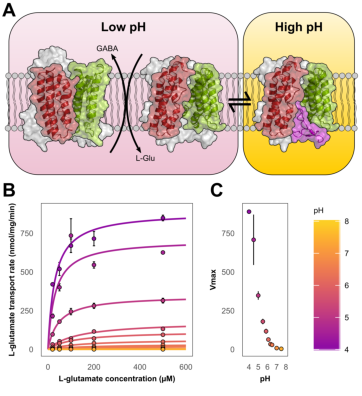
\includegraphics[width=3.25in]{Figures/gadc_main_transport.pdf}
 \caption[Transport activity in the glu/GABA antiporter GadC is dependent on pH.]{Transport activity in the glu/GABA antiporter GadC is dependent on pH. (A) Cartoon depiction of the activation mechanism. (B) Glutamate transport in wildtype GadC reconstituted into proteoliposomes is strongly dependent on pH. (C) Maximal transport rate (Vmax) increases exponentially as a function of pH.}
\label{fig:gadc_main_transport}
\end{wrapfigure}
	
The pH-dependent activity profile of GadC was verified by measuring radiolabeled substrate uptake into proteoliposomes. A construct of wildtype GadC, previously cloned from \emph{E. coli} str. O157:H7, was obtained and expressed in \emph{E. coli} C43 (DE3), purified in $\mathrm{\upbeta}$-DDM detergent micelles, and reconstituted into proteoliposomes containing \SI{5}{mM} \gls{glu} at pH 5.5. These proteoliposomes were then tested for substrate transport by detection of [$\mathrm{^3H}$]-L-glutamic acid uptake as a function of both external pH and substrate concentration. Additionally, time-dependent \gls{glu} transport was measured in proteoliposomes containing \SI{5}{mM} \gls{gaba} at pH 5.5 (Figure \ref{fig:gadc_supp_time_transport}). Consistent with previous findings \citep*{Ma2013, Ma2012, Tsai2013}, we observed a strong dependence of radioligand uptake on pH, with negligible transport detected at pH 6.5 and above (Figures \ref{fig:gadc_main_transport}.B and C).

To characterize the structural changes associated with pH-dependent activation, we used site-directed spin labeling and \gls{epr} spectroscopy \citep*{Jeschke2012, Mchaourab2011}. After mutating all three endogenous cysteines in the wildtype sequence to chemically inert residues (C60V, C247A, C380V), a panel of 25 single- and double-cysteine mutants were generated. As with previous studies on structural homologs of GadC, double-cysteine pairs were selected based on their ability to report on inter- and intra-domain motions. To evaluate if these measurements were expected to fall within the detectable range for DEER measurements (\SIrange{15}{60}{\angstrom}) and to test whether the resulting data were consistent with the crystal structure, distance measurements were first simulated between candidate residue pairs using dummy spin labels modeled over the crystal structure \citep*{Islam2013, Jo2014}. Following purification and spin-labeling, all mutants were reconstituted into proteoliposomes and tested for transport and pH-dependent inactivation at pH 5.5 (Figure \ref{fig:gadc_supp_transport}) and 7.5 (Figure \ref{fig:gadc_supp_transport75}), respectively. Additionally, all experimental \gls{deer} measurements were carried out in nanodiscs with lipid profiles matching those of the proteoliposomes used for transport assays. This ensured that neither the spin labels nor the membrane environment interfered with the protein's ability to traffic substrates at acidic pH or to undergo inactivation at neutral pH.


\begin{wrapfigure}{r!}{0.5\textwidth}
\centering
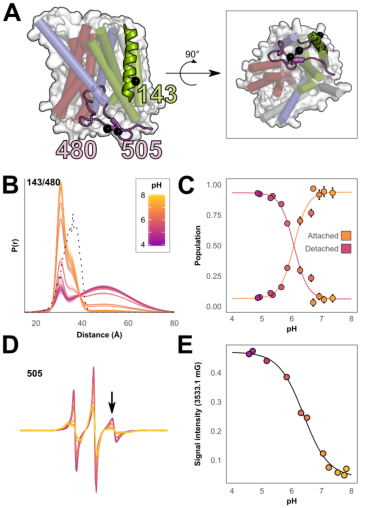
\includegraphics[width=3.25in]{Figures/gadc_main_tail.pdf}
 \caption[Detachment of the C-terminus is triggered by low pH.]{Detachment of the C-terminus is triggered by low pH. (A) Position of the C-terminus, shown in pink, relative to the main transmembrane domain of the transporter. Inset: The domain is embedded into the intracellular vestibule. (B) At low pH, a distance component consistent with a distance distribution predicted from the crystal structure (shown in the dashed line) is replaced by a wider, longer-distance component. (C) Titration measurement of the dissociation of the C-terminus. (D) pH-dependent increases in conformational heterogeneity resolved by CW-\gls{epr}. (E) Titration measurement of the third moment of the CW spectra reveals a similar profile to the DEER measurements.}
\label{fig:gadc_main_tail}
\end{wrapfigure}

Although GadC was crystallized as an antiparallel homodimer, no experimental evidence of this quaternary assembly was detected in lipid nanodiscs (shown below). Additionally, the addition of substrates induced neither large-scale conformational modulations nor changes in continuous-wave \gls{epr} lineshape data (representative pairs shown in Figure \ref{fig:gadc_supp_substrates}). As a result, the following discussion is limited to pH-dependent structural changes.

\subsection{Monitoring the detachment of the C-terminus as a function of pH}


Abrogation of transport at neutral and alkaline pH has previously been attributed to a coiled domain at the protein's extreme C-terminus (shown in pink in Figures \ref{fig:gadc_main_transport} and \ref{fig:gadc_main_tail}.A). In the crystal structure of GadC, captured at pH 8.0, this domain is embedded in the intracellular cavity and putatively obstructs closure of the intracellular gate, a prerequisite of alternating access. To test the hypothesis that this domain detaches under acidic conditions, a double-cysteine mutant (143C/480C) was generated and spin-labeled to measure the distance between the C-terminus and the transmembrane domain.  Distance distributions of this pairs reported large changes as a function of pH.  At neutral pH, the average distance matched that predicted from the crystal structure, whereas a sharp increase in both the magnitude and the width of the distribution was observed under acidic conditions (Figure \ref{fig:gadc_main_tail}.B, raw data shown in Figure \ref{fig:gadc_supp_tail}). A nonlinear least-squares fit of a sigmoid function to the amplitudes of the short- and long-distance components revealed that this shift occurred cooperatively with a pKa of 6.07±0.11 (Figure \ref{fig:gadc_main_tail}.C), with both short-distance components diminishing at low pH in a tightly correlated manner (Figure \ref{fig:gadc_supp_tail_rsq}).

To further determine if this cooperative distance change originated from  conformational disorder of the C-terminal domain, a second single-cysteine mutant was introduced near the C-terminal extreme of the domain (505C). At neutral pH, the lineshape of this mutant's \gls{cw}-\gls{epr} spectrum suggested that the domain was relatively structured, consistent with its docked conformation in the crystal structure. By contrast, reducing the pH led to a sharp spectral component that dominated the lineshape at pH 6.0 and below, suggesting increases in the C-terminal domain's disorder and mobility. Nonlinear least squares fit of the signal's intensity of the high field line on as a function of pH yielded a pKa of 6.30±0.04, consistent with the \gls{deer} measurements discussed above (Figure \ref{fig:gadc_main_tail}.D and E). Taken together, the data are consistent with the corroborate the hypothesis that the tail detaches from the transmembrane domain and becomes heterogeneous and disordered. Additionally, the pKa of this event closely matched the pH at which transport activity is abrogated, reinforcing this domain’s role in regulating substrate exchange under neutral pH conditions.
	
\subsection{Characterization of structural changes in the transmembrane domain induced by low pH}

To determine if low pH drives additional structural changes following detachment of the C-terminal domain, a systematic analysis of the structure of GadC was undertaken. A variety of motifs defining conformational heterogeneity and alternating access have been observed in structural homologs using both high-resolution methods, such as crystallography and \gls{cryoem} \citep*{Bozzi2019, Kazmier2017, Krishnamurthy2012, Lee2019, Liu2019, Perez2012, Shimamura2010,  Weyand2008, Yamashita2005, Yan2019}, as well as solution-state methods such as \gls{epr} spectroscopy \citep*{Claxton2010, Kazmier2014, Kazmier2014a, Paz2018}, \gls{fret} \citep*{Zhao2010}, and \gls{hdxms} \citep*{Adhikary2017, Merkle2018, Moeller2019, Nielsen2019}. Depending on the transporter, isomerization between inward- and outward-facing conformations appears to be largely mediated by combinations of rigid-body movements between the bundle and hash domains, movement of \gls{el}2 and unwinding of \gls{tmh}5, and/or independent movement of \gls{tmh}1, \gls{tmh}6a, \gls{tmh}7, and/or \gls{el}4. We thus set out to test if movement in these motifs underpin activation of GadC at low pH.
	
\subsection{The bundle domain is tilted relative to the crystal structure}

\begin{figure}[h!]
\centering
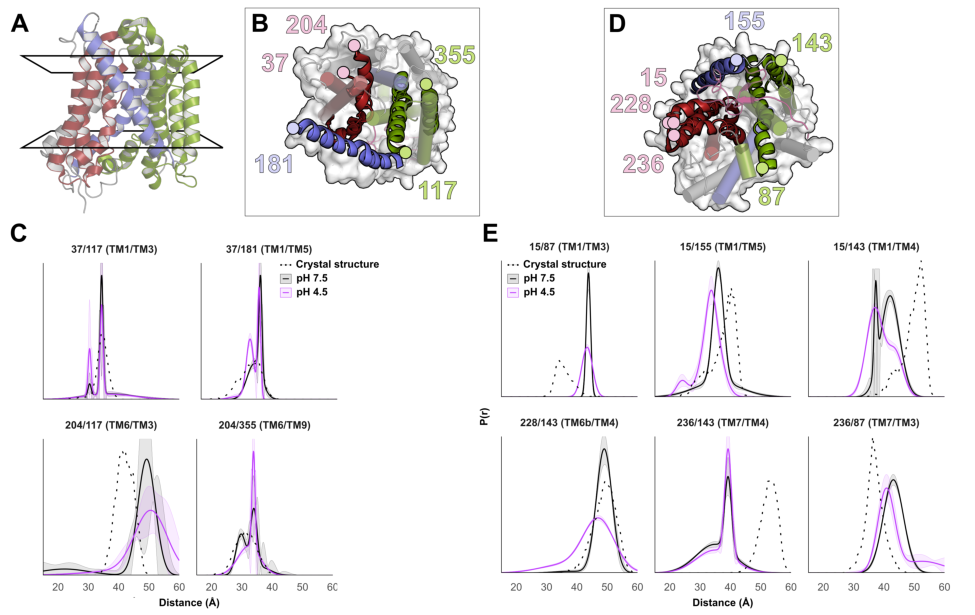
\includegraphics[width=6.5in]{Figures/gadc_main_bundle_hash.pdf}
 \caption[Distance measurements between the bundle and scaffold domains reveal deviate from crystal structure.]{Distance measurements between the bundle and scaffold domains deviate from crystal structure. (A) Side view of GadC with the top and bottom slices corresponding to panels B and D, respectively. (C) Distance measurements carried out at pH 4.5 and 7.5 alongside predictions made from the crystal structure. Confidence intervals (95\%) shown as shaded regions. (E) Distance measurements on the intracellular side reveal striking inconsistencies with the crystal structure.}
\label{fig:gadc_main_bundle_hash}
\end{figure}

A series of measurements were carried out between spin labels attached to the bundle domain and either the hash domain or \gls{tmh}5 on the extracellular side of the GadC (Figure \ref{fig:gadc_main_bundle_hash}.A). Distance distributions collected at pH 7.5 were largely in agreement with predictions made from the crystal structure, in which the extracellular gate was fully closed (Figure \ref{fig:gadc_main_bundle_hash}.B). Consistent with this finding, \gls{cw} profiles involving residue 37, located on the loop connecting helices 1 and 2, were broad and indicative of a constrained environment (Figure \ref{fig:gadc_supp_bundle_hash_extra}). Additionally, cysteine mutants labeled at this residue showed partially abrogated transport at low pH (Figure \ref{fig:gadc_supp_transport}). Only minor changes were observed in measurements at pH 4.5, suggesting that the extracellular vestibule remained closed even at low pH. Although broadening was observed between \gls{tmh}3 and \gls{tmh}6, the considerable overlap between the 95\% confidence intervals for both distributions prevented us from definitively concluding that this resulted from conformational rearrangements. The remainder of the data indicate that at both low and high pH, the extracellular gate is consistent with the outward-closed conformation observed in the crystal structure (Figure \ref{fig:gadc_main_bundle_hash}.C).

In contrast to these observations, distance measurements carried out on the intracellular side of GadC deviated substantially from predictions made from the crystal structure (Figures \ref{fig:gadc_main_bundle_hash}.D, \ref{fig:gadc_main_bundle_hash}.E, and \ref{fig:gadc_supp_bundle_hash_intra}). At pH 7.5, we observed that \gls{tmh}1 and \gls{tmh}7 in the bundle domain were \SIrange{10}{15}{\angstrom} farther from \gls{tmh}3, and \SIrange{10}{20}{\angstrom} closer to \gls{tmh}4 and \gls{tmh}5, than the predictions made from the crystal structure. Lowering the pH to 4.5 caused these distance distributions to broaden and, in some distributions, to further shorten by \SIrange{3}{5}{\angstrom}. However, the pairwise nature of the data do not immediately indicate which regions of the protein A) deviated from the crystal structure, and B) underwent increases in heterogeneity.

\subsection{The scaffold domain is largely consistent with the crystal structure}

As only minor pH-dependent movement was observed between the bundle and hash domains, subsequent measurements focused on \gls{el}4 and \gls{il}1, which connected helices 7 and 8 and 2 and 3, respectively. \Gls{el}4 has been shown to pivot outward and provide access to the extracellular vestibule in LeuT \citep*{Claxton2010, Kazmier2014a}, whereas transport activity data suggest that \gls{il}1 is involved in mediating pH-dependent activation in the homolog AdiC \citep*{Wang2014}. In addition to revealing whether the positions of these domains respond to changes in pH, the \gls{deer} data could further determine the extent to which the discrepancies observed between our measurements and predictions made from the crystal structure extended to the remainder of the structure.

\begin{figure}[h!]
\centering
\includegraphics[width=6.5in]{Figures/gadc_main_il1_el4.pdf}
 \caption[No pH-dependent movements are observed in IL1 and EL4.]{No pH-dependent movements are observed in IL1 and EL4. (A) Extracellular view of GadC. (B) Measurements between EL4 and extracellular sites on the scaffold domain suggest that TM5 is closer to the main body of the transporter than in the crystal structure. Confidence intervals (95\%) shown as shaded regions. (C) Intracellular view of GadC. (D) Intracellular measurements within the scaffold domain. (D) Intracellular view. (E) Side view. (F) In-to-out measurement suggests a slight pH-dependent movement in \gls{tmh}9.}
\label{fig:gadc_main_il1_el4}
\end{figure}

On the extracellular side, we collected three distance distributions between \gls{el}4 and various points in the structure (Figures \ref{fig:gadc_main_il1_el4}.A, \ref{fig:gadc_main_il1_el4}.B, and \ref{fig:gadc_supp_el4}). None of the distributions indicated a large-amplitude distance change as would be expected from \gls{el}4-mediated opening of the extracellular vestibule. However, whereas two of the distributions involving the C-terminal end of \gls{el}4 (residue 280) were in reasonable agreement with the crystal structure, a third pair collected between \gls{tmh}5 and \gls{el}4 showed a shorter-than-expected distance distribution. To ascertain if this discrepancy was due to the position of \gls{tmh}5, rather than \gls{el}4, we collected an additional measurement between TM3 and TM5 and found that it too was also shorter than expected (Figure \ref{fig:gadc_main_il1_el4}.A). A likely explanation is that the extracellular side of \gls{tmh}5 does not protrude as far as suggested by the crystal structure, and that the position of \gls{el}4 is otherwise consistent with the crystal structure.

Distance distributions between \gls{il}1 and \gls{tmh}3 similarly showed little movement and suggest that the two helices are effectively stapled together, consistent with a lack of independent movement observed in other LeuT-fold transporters (Figures \ref{fig:gadc_main_il1_el4}.C, D, and \ref{fig:gadc_supp_il1}). Further measurements across the hash domain on the intracellular side highlight its structural invariance. However, minor pH-dependent distance changes in \gls{il}1/\gls{tmh}4 are observed and appear to accompany local reconfigurations as evidenced by the \gls{cw} profile (Figure \ref{fig:gadc_supp_il1}). Alongside evidence that other distributions involving residue 143 on \gls{tmh}4 were bimodal, these data suggest that several distinct nitroxide rotamer states may be populated and that their relative proportions shift as a function of pH. Measurements from the hash domain to \gls{tmh}5, by contrast, do indicate minor changes in their relative positions. This further illustrates how changes in pH and detachment of the C-terminal tail domain coincide with subtle reorganizations of helices on the intracellular side of the protein.

Interestingly, measurements between \gls{il}1 and \gls{tmh}9 on the extracellular side suggested a slight sharpening that may be pH-dependent (Figure \ref{fig:gadc_main_il1_el4}.E and F). The similarity in the distance changes observed between both \gls{tmh}6/\gls{tmh}9 (204/355) and \gls{el}4/\gls{tmh}9 (280/355; Figures \ref{fig:gadc_main_bundle_hash}.A and \ref{fig:gadc_main_il1_el4}.A, respectively), combined with the lack of distance changes in measurements involving IL1, suggest that these data as slight pH-dependent movements of \gls{tmh}9. However, this movement is substantially less than what is observed in structural homologs, such as Mhp1 \citep*{Shimamura2010, Weyand2011, Weyand2008}, that use the loop connecting \gls{tmh}9 and \gls{tmh}10 as a hinge to facilitate entry and exit from the substrate-binding site.

Altogether, the data reveal minor structural rearrangements on the intracellular side but fail to precisely identify which domains are moving and which are stationary.

\subsection{The bundle domain does not behave like a rigid body}

Finally, we evaluated whether the bundle domain acted as a rigid body during this pH transition. The narrowness of this domain, combined with the \SI{15}{\angstrom} lower limit of \gls{deer}, meant that we could only answer this question using distance measurements between the intracellular and extracellular sides of the protein (Figure \ref{fig:gadc_main_bundle_only}.A). Distance changes were observed in every measurement (Figures \ref{fig:gadc_main_bundle_only}.A and \ref{fig:gadc_supp_bundle_only}), arguing against the possibility that this domain acts as a rigid body as previously posited. Additionally, they reveal minor discrepancies regarding the position of the extracellular half of \gls{tmh}6, which was hinted at by measurements described previously involving the hash domain (Figure \ref{fig:gadc_main_bundle_hash}.A).

\begin{wrapfigure}{r!}{0.5\textwidth}
\centering
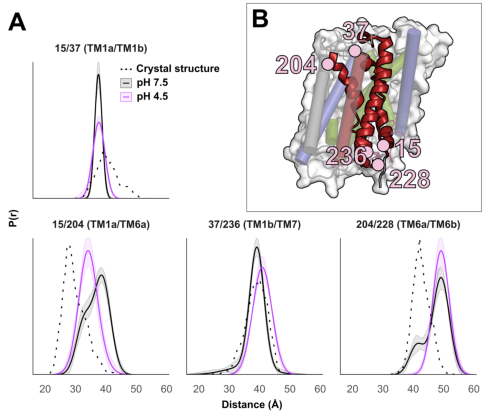
\includegraphics[width=3.25in]{Figures/gadc_main_bundle_only.pdf}
 \caption[Measurements within the bundle domains are inconsistent with a rigid-body pattern of conformational dynamics. ]{Measurements within the bundle domains are inconsistent with a rigid-body pattern of conformational dynamics. (A) In-to-out \gls{deer} distance distributions in the bundle domain. Confidence intervals (95\%) shown as shaded regions. (B) Side view showing the measurements.}
\label{fig:gadc_main_bundle_only}
\end{wrapfigure}

\subsection{GadC adopts an inward-facing occluded conformation at both pHs}

To summarize the experimental \gls{deer} data, we observed both substantial deviations between our observations and predictions made from the crystal structure, as well as minor pH-dependent broadening and amplitude changes. To translate these pairwise measurements into fold-level structural models, we generated a series of structural models of GadC using the modeling software suite Rosetta \citep*{Leaver-fay2011, Leman2020}. Unfortunately, high-precision models of the structure of GadC cannot be obtained given the relatively small number of available distance restraints. Therefore, we supplemented the modeling process with a custom-designed statistical potential that quantified each model's similarity to the structures of previously determined homologs. The design of this potential, outlined in Section \ref{sec:gadc_methods},  capitalized on the large number of structures of homologs deposited in the Protein Databank. Effectively, this statistical potential served as a form of regularization to penalize the introduction of conformational changes that are not anticipated by the known structures of closely related homologs of GadC.

We generated 5,000 Rosetta models for each pH condition using a procedure discussed in detail in section \ref{sec:gadc_methods} and Appendix \ref{app:confchangemover}. Experimental \gls{deer} data was introduced as distance restraints using the RosettaDEER module (Chapter \ref{ch:rosettadeer}) and the scoring function discussed in Appendix \ref{app:scoring}. Each model generated this way was reweighed based on its structural similarity to homologous transporters (discussed in section \ref{sec:leutintro_antiporters}). The five best-scoring models generated using data collected at either pH are shown in Figures \ref{fig:gadc_main_model}.A and \ref{fig:gadc_supp_models}. These models principally deviated from the crystal structure in the positions of \gls{tmh}1 and 7, although we note that the hash domain adopted a slightly more "upright" conformation with \gls{tmh}4 nearly parallel to the membrane normal. By contrast, the extracellular sides of these models closely resembled that of GadC, with subtle modifications to \gls{tmh}5 and \gls{tmh}6a. Initial structural comparisons suggest that these models resemble the inward-facing occluded conformation of the homologs ApcT \citep*{Shaffer2009} and MjApcT \citep*{Jungnickel2018}, in which the bundle domain is tilted toward \gls{tmh}4 and away from \gls{tmh}3 relative to the crystal structure of GadC as suggested by the data (Figure \ref{fig:gadc_main_model}). However, unlike ApcT, \gls{tmh}5 in our models is not bent or puckered and instead adopts a configuration similar to that observed in the GadC crystal structure. In fact, despite differences in the bundle domain, the overall structure of our models closely resembles the structure of GadC, highlighting both the data's limited disagreement with the crystal structure and the effectiveness of our regularization strategy.

\begin{figure}[h]
\centering
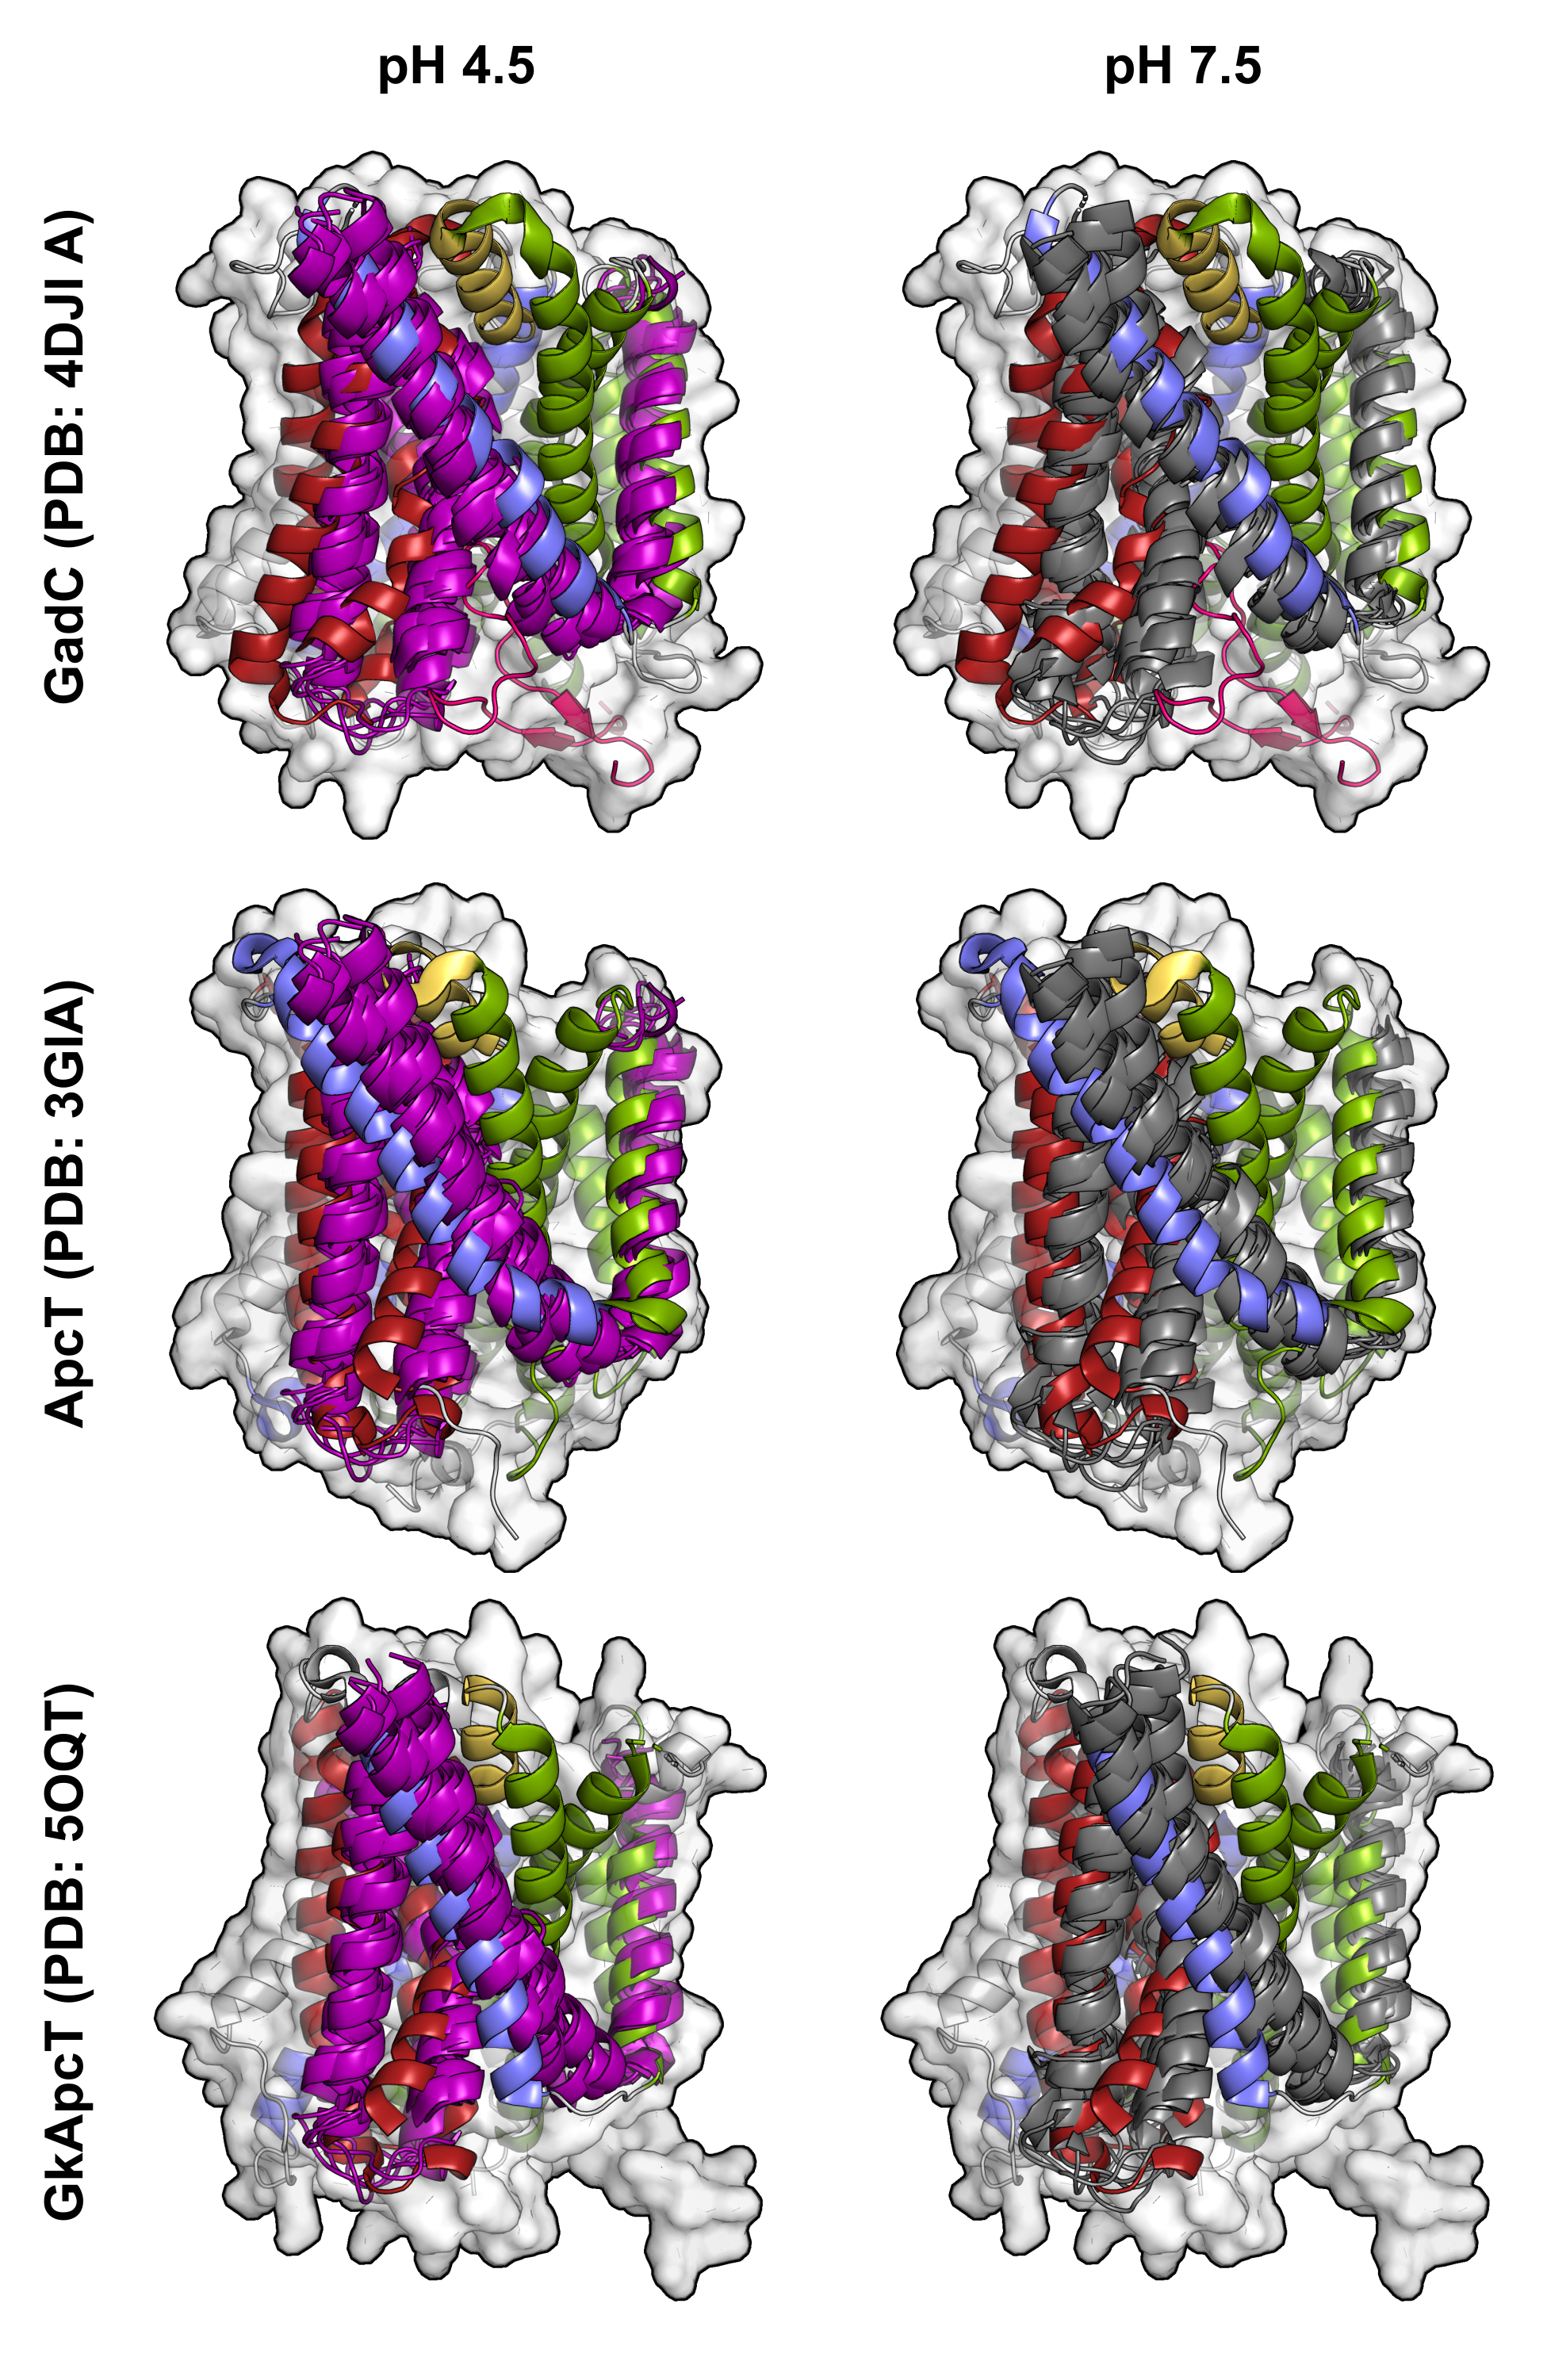
\includegraphics[width=3.25in]{Figures/gadc_main_model.pdf}
 \caption[Rosetta models of the low- and high-pH conformations generated using the DEER data in purple and dark grey, respectively.]{Rosetta models of the low- and high-pH conformations generated using the DEER data in purple and dark grey, respectively. Crystal structures of GadC and its homologs ApcT and GkApcT are shown in the colored helices and suggest that GadC adopts an inward-facing occluded conformation.}
\label{fig:gadc_main_model}
\end{figure}

These clear deviations from the crystal structure contrasted with far more subtle differences observed between low-pH and high-pH models. In fact, although small pH-dependent distance changes were observed in the data, variation between the top five models at either pH were comparable to differences between models across different pHs (Figure \ref{fig:gadc_supp_models}). Therefore, we conclude that the resolution and sparseness of the data prevent the structural basis of pH-dependent activation following release of the C-terminus from being determined with high confidence. It is therefore unclear if increases in heterogeneity observed at low pH are the result of movement in \gls{tmh}5, as suggested by structures of homologous transporters, or \gls{tmh}1, which is more strongly supported by the \gls{deer} data. 

\section{Discussion}\label{sec:gadc_discussion}

The \gls{deer} data presented here investigates the structure and dynamics of the pH dependent \gls{glu}/\gls{gaba} antiporter GadC at low pH. These measurements, which reflect solution-state backbone dynamics \citep*{Jeschke2012, Kazmier2017}, are inconsistent with the conformation stabilized by the crystal lattice, with substantial deviations observed on the intracellular side of the protein. Instead, models generated using Rosetta suggested that GadC adopts a conformation similar to closely related homologs in which its the intracellular vestibule of GadC is partially occluded and resemble the inward-facing occluded conformations observed in the closely related homologs. Indeed, we found that a model of GadC generated \emph{de novo} using the state-of-the-art method RoseTTAFold \citep*{Baek2021} generated a similarly \gls{if}-occluded model that was more consistent with the data than the crystal structure \ref{fig:gadc_supp_rosettafold}. This conformation is all the more notable given the crystal structure's similarity to homologs such as BasC \citep*{Errasti-Murugarren2019}, Lat-1 \citep*{Lee2019, Yan2019}, Lat-2 \citep*{Yan2020}, and $\mathrm{b^{(0,+)}AT1}$ \citep*{Wu2020, Yan2020a}. It should be noted, however, that our measurements reflect the structure and dynamics of GadC in a more physiologically relevant lipid environment. The aforementioned homologs, by contrast, were structurally characterized in detergent micelles and/or when bound to antibodies. It should be noted that lipid/detergent-dependent conformational changes have also been reported in several transporters, including the structural homolog LeuT \citep*{Quick2009, Sohail2016}, as well as other membrane proteins. 

The absence of substrate-induced conformational changes observed at low pH (Figure \ref{fig:gadc_supp_substrates}) contrasts with results from similar studies of unrelated antiporters, such as those mediating sodium- or proton-dependent drug efflux. However, this discrepancy may be explained by the fact that, unlike the substrates of ion coupled antiporters, neither glutamate nor GABA are hypothesized to move down their concentration gradients under physiological conditions. This owes to bacterial responses to acid stress that trigger rapid decarboxylation and depletion of cytoplasmic amino acids, such as glutamate, and the corresponding spike in cognate polyamines, such as GABA \citep*{Foster2004, Richard2004}. In fact, all four of the "virtual proton pumps" involved in bacterial acid resistance, including GadC, are co-transcribed with corresponding amino acid decarboxylases \citep*{Kanjee2013}. This metabolomic adaptation ensures that neither half of GadC's transport cycle, glutamate import or GABA export, is energetically unfavorable. This, in turn, may would obviate the need for ligand-dependent changes in thermodynamics equivalent to, for example, the pH-dependent conformational rearrangements observed in proton/drug antiporters \citep*{Dastvan2016a, Jagessar2020, Masureel2014}.

On the basis of this observation, we propose a model in which the transport cycle of GadC consists of two half-cycles of uniport in which facilitated diffusion of both \gls{glu} and \gls{gaba} are coupled in opposite directions (Figure \ref{fig:gadc_main_transportmodel}). This posits that substrate binding contributes to the kinetics, rather than the thermodynamics, of the transporter's functional cycle. We propose that this is achieved by stabilization of a high-energy transition state separating the inward-facing and outward-facing conformations that, under apo conditions, cannot be traversed. Ligand-induced increases in conformational flexibility, which would be consistent with this hypothesis, have previously been reported in the homologous serine/threonine exchanger SteT using single-molecule dynamic force spectroscopy \citep*{Bippes2009}. These findings could extend to homologous amino acid exchangers in humans, such as xCT, which couples the energetically favorable export of glutamine to the import of cystine, which is immediately reduced to two cysteine molecules and thus absent from the cytoplasm \citep*{Oda2020}.

\begin{figure}[h!]
\centering
\includegraphics[width=3.75in]{Figures/gadc_main_transportmodel.pdf}
 \caption[Mechanistic model of pH-dependent activation and substrate transport in GadC.]{Mechanistic model of pH-dependent activation and substrate transport in GadC. (A) Under acidic conditions, the C-terminal domain of GadC detaches. Separately, GadB decarboxylates intracellular glutamate into GABA, consuming protons and increasing intracellular pH. (B) GadC undergoes two half-cycles of energetically downhill uniport. High cytoplasmic concentrations of GABA ensure that its export is the most energetically favorable means of undergoing \gls{if}-to-\gls{of} isomerization, while low cytoplasmic concentrations of glutamate ensure that its import is the most energetically favorable means of undergoing \gls{of}-to-\gls{if} isomerization.}
\label{fig:gadc_main_transportmodel}
\end{figure}

Nevertheless, as these conclusions are derived from data collected under equilibrium conditions, they do not reflect structural changes induced by  substrate in the presence of gradients, such as those reported in structural homologs such as SGLT1 \citep*{Loo1998}. The possibility that the conformational dynamics of \gls{apc} transporters are responsive to gradients is reinforced by evidence that homologous transporters preferentially bind substrates on specific sides of the membrane \citep*{Bartoccioni2019}. For this reason, further inquiries must determine the structure and function of GadC as it operates in and maintains a pH gradient.

\section{Materials and Methods}\label{sec:gadc_methods}

\subsection{Site-directed mutagenesis}

A codon-optimized version of the GadC gene from \emph{Escherichia coli} str. O157:H7 (Genscript) was cloned into a pET19b vector encoding an N-terminal deca-histidine tag. A cysteine-less construct (C60V, C246A, C380V) was generated from this template using site-directed mutagenesis (QuikChange). All single- and double-cysteine mutants were similarly generated from this cysteine-free construct and verified by Sanger sequencing using both T7 forward and reverse primers.

\subsection{Expression, purification, and spin labeling of GadC}

Plasmids encoding either wildtype or mutant GadC were transformed into competent \emph{E. coli} str. C43 (DE3) cells and overexpressed in 1L minimal media A supplemented with ampicillin (Gold Biotechnology) as previously described60. Upon reaching an absorbance (OD600) of 0.7-0.8, GadC expression was induced by adding \SI{1}{mM} IPTG (Gold Biotechnology) and the temperature was dropped to 20°C. Cells were harvested after 16 hours by centrifugation at \SI{5500}{g} for 15 minutes, resuspended in \SI{22}{mL} lysis buffer (\SI{100}{mM} KPi, \SI{10}{mM} DTT, pH 7.5), and lysed by sonication. After centrifugation at \SI{9000}{g} for 15 minutes, the supernatant was collected and ultracentrifuged at \SI{200000}{g} for \SI{90}{minutes}.

The pelleted membrane fractions were then solubilized in resuspension buffer (\SI{50}{mM} Tris/Mes, \SI{200}{mM} NaCl, 20\% glycerol, \SI{1}{mM} DTT, pH 7.5) containing 1\% $\mathrm{\upbeta}$-DDM (Anatrace) and stirred on ice for \SI{60}{minutes}. Insoluble material was removed by ultracentrifugation at \SI{200,000}{g} for \SI{30}{minutes}, and the supernatant was incubated with \SI{1.0}{mL} Ni-NTA Superflow (Qiagen) resin at 4°C for two hours with \SI{25}{mM} imidazole. After washing with ten column volumes of resuspension buffer containing \SI{50}{mM} imidazole and 0.05\% B-DDM, purified GadC was eluted from the resin using resuspension buffer with \SI{250}{mM} imidazole and 0.05\% β-DDM.

Following the addition of \SI{60}{mM} Mes, single- and double-cysteine mutants were labeled with three rounds of 20-fold molar excess \gls{mtssl} (Enzo Life Sciences) per cysteine at room temperature and moved to ice overnight after four hours. Samples were then concentrated using Amicon Ultra \SI{50,000}{MWCO} filter concentrators (Millipore) to a final concentration no greater than \SI{3}{mg/ml}, as reported by absorbance at \SI{280}{nm} ($\epsilon$=\SI{67,840}{M^{-1}.cm^{-1}}), and purified into \SI{200}{mM} Tris/Mes, pH 7.2, 20\% glycerol, 0.05\% $\mathrm{\upbeta}$-DDM by size exclusion chromatography using a Shodex KW-803 column with guard column. Peak fractions were isolated for further studies.

\subsection{Reconstitution of GadC into proteoliposomes}

A 3:1 ratio (weight/weight) of \emph{E. coli} polar lipids and L-$\mathrm{\upalpha}$-phosphocholine (Avanti Polar Lipids) were dissolved in chloroform and evaporated with a rotary evaporator. After overnight desiccation in a vacuum chamber, lipids were resuspended in the appropriate buffer, homogenized by ten cycles of freeze-thawing, and stored in small aliquots at -80°C.

Lipids prepared for liposomes were resuspended in \SI{25}{mM} KPi, \SI{150}{mM} KCl pH 5.5, and either \SI{5}{mM} L-Glu or \SI{5}{mM} \gls{gaba} to a final concentration of \SI{20}{mg/ml} (\SI{16.4}{mM}). Before reconstitution, lipids were diluted and destabilized with the addition of 1.25\% \gls{bog} (Anatrace) and extruded through a \SI{400}{nm} membrane filter (Whatman). Purified GadC was added to the sample at a 1:200 ratio (weight/weight), bringing the final lipid concentration to \SI{5}{mg/mL}. Following a thirty-minute incubation at room temperature, detergent was removed from the sample by the gradual addition of \SI{400}{mg/mL} SM-2 polystyrene Bio-Beads (Bio-Rad) over the course of four hours. After rocking overnight in the dark, the proteoliposome solution was cleared of biobeads and ultracentrifuged at \SI{150,000}{g} for \SI{60}{minutes}. Proteoliposomes were then resuspended in external buffer (\SI{25}{mM} KPi, \SI{150}{mM} KCl, pH 5.5) and ultracentrifuged to remove external substrates. After repeating this ultracentrifugation step a total of three times, proteoliposomes were suspended in external buffer at a final lipid concentration of \SI{100}{mg/ml}. GadC concentration was then quantified using SDS/PAGE and densitometry (ImageJ v. 1.53g), with purified GadC in $\mathrm{\upbeta}$-DDM serving as a standard curve.

\subsection{Transport assays}\label{sec:gadc_transport_assay}

\emph{In vitro} transport assays were carried out either in triplicate (concentration-dependent) or in duplicate (time-dependent) as previously described \citep*{Ma2012}. An additional baseline measurement was performed on ice. Glutamic acid (between \SI{25}{\upmu M} and \SI{1}{mM}) was added to external buffer and checked for pH immediately prior to all transport experiments. For the time-dependent transport \gls{glu}/\gls{gaba} exchange assays shown in Figure \ref{fig:gadc_supp_time_transport}, an fixed external \gls{glu} concentration of \SI{50}{\upmu M} at pH 5.5 was used. In both experiments, proteoliposomes (\SI{2}{\upmu L}) were added to external buffer (\SI{98}{\upmu L}) containing \SI{1}{\upmu Ci} [$\mathrm{^3H}$]-L-glutamic acid (approximately \SI{200}{nM}) and gently agitated. For titration experiments on wildtype GadC, proteoliposomes (\SI{1}{\upmu L}) were added to external buffer (\SI{99}{\upmu L}) containing \SI{1}{\upmu Ci} [$\mathrm{^3H}$]-L-glutamic acid. Substrate uptake proceeded for two minutes at 25°C and was quenched by adding ice-cold stop buffer (\SI{25}{mM} glycine, \SI{150}{mM} KCl, pH 9.5) and vacuum-filtering the solution through a \SI{0.22}{\upmu m} GSTF filter (Millipore) pre-soaked in stop buffer. The filter was then washed with an additional \SI{6}{mL} stop buffer, removed, and added to \SI{5}{mL} Ecoscint H scintillation solution (National Diagnostics). Following quantitation, data were analyzed using Michaelis-Menten kinetics using the \emph{curve\_fit} function implemented in SciPy \citep*{Virtanen2020}. Baseline measurements were subtracted from the 25°C measurements.

\subsection{Reconstitution of GadC into lipid nanodiscs}

Lipids for nanodisc reconstitution were prepared as described above and resuspended in \SI{50}{mM} Tris/Mes pH 7.5 to a final concentration of \SI{20}{mM}. MSP1D1E3 was purified as previously described \citep*{Jagessar2020}. Nanodisc reconstitution proceeded using a molar ratio of 1:8 GadC:MSP1D1E3, 1:50 MSP1D1E3:lipid, and 1:5 lipid:cholate. Detergents were gradually removed from the solution using SM-2 Bio-Beads as previously described \citep*{Jagessar2020}. After overnight incubation, biobeads were removed from the solution using a \SI{0.20}{\upmu m} filter. Nanodisc-reconstituted GadC was then isolated from empty nanodiscs by size-exclusion chromatography using a Superdex 200 Increase 10/300 GL column into \SI{50}{mM} Tris/Mes, pH 7.5, 10\% glycerol and concentrated using an Amicon Ultra \SI{100,000}{MWCO} filter concentrator (Millipore). The pH of all protein samples was carefully determined using a microelectrode and adjusted using \SI{1}{M} citrate and \SI{1}{M} Tris. Protein concentration was then evaluated using \gls{cw} \gls{epr} spectroscopy as previously described \citep*{Zou2010}. Glycerol was added to all \gls{deer} samples to a final concentration of 23\% vol/vol, which were then flash-frozen in liquid nitrogen prior to DEER spectroscopy.

\subsection{CW-EPR and DEER spectroscopy and data analysis}

Spin-labeled GadC was characterized using \gls{cw}-\gls{epr} at 25°C using a Bruker EMX spectrometer operating at a frequency of \SI{9.5}{GHz}, a \SI{10}{mW} incident power, and a modulation amplitude of \SI{1.6}{G}. \Gls{deer} measurements were carried out using a dead-time free four-pulse protocol \citep*{Pannier2000} at either \SI{50}{K} (for 143C/480C) or \SI{83}{K} (all other double-cysteine mutants). Pulse lengths were as follows: \SIrange{10}{14}{ns} (first $\frac{\pi}{2}$ pulse), \SI{20}{ns} (second and fourth $\pi$ pulse), and \SI{40}{ns} (third $\pi$ pulse). The pump and observation frequencies were separated by \SI{62.26}{MHz}. Echo decay data were analyzed into distance distributions using GLADDvu with the last \SI{500}{ns} of the signal truncated \citep*{Hustedt2018}. Fitting model parameters were chosen using the Bayesian Information Criterion. To analyze the pH titration distance data collected using GadC 143C/480C, the long-distance component was isolated from the two short-distance components, and was fitted with a sigmoid function using the \emph{curve\_fit} function as implemented in SciPy \citep*{Virtanen2020}. For all \gls{deer} pairs, the distance distributions were compared to predictions generated by MDDS, which was accessed using the CHARMM-GUI web server \citep*{Jo2014}.

\subsection{Generation of a structure-based statistical potential}\label{sec:gadc_potential}

After manually isolating the ten core transmembrane helices defining the LeuT-fold, each protein was aligned to each other using TM-Align version 20180426 \citep*{Zhang2005}. For each model, the highest TMscore \citep*{Zhang2004} to a transporter in the \gls{apc} family was obtained. TMscore quantifies structural similarity and ranges from 0 to 1, with 1 indicating perfect structural overlap \citep*{Xu2010}; values between different structures of the same transporter were not considered. To reflect the probability of a model belonging to the \gls{apc} family given its TMscore to structures of other proteins in that family, we used the following exponential function:

\begin{equation}
    p(M)=\exp \left( -\frac{1\mathrm{-}TMscore}{\upbeta} \right)
\end{equation}
This function was parametrized by minimization of the total cross-entropy $-\sum{\ln \left(q_i\right)}$, where $q_i=p(M_i)$ for all \gls{apc} transporters and $q_i=1-p(M_i)$ for all non-\gls{apc} LeuT-fold transporters. Using the \emph{minimize} function implemented in SciPy \citep*{Virtanen2020}, a value of $\upbeta=0.072185$ was obtained.

\subsection{Initial homology modeling}

Structural alignments were obtained using TMAlign. The Rosetta application \emph{partial\_thread} was then used to thread the first ten transmembrane helices (residues 1-359) of the GadC sequence over each structure. The three remaining helices were then directly grafted onto the structure by structural alignment; the C-terminal tail (residues 471-511) was omitted. Homology models were constructed using HybridizeMover \citep*{Song2013} with five randomly selected templates as well as the hash domain from GadC (PDB: 4DJI chain A). The weight of the \gls{deer} data was set to 10.0 during the first two stages and to 0.0 during the final full-atom minimization stage. Sequence fragments used during this step were obtained from the Robetta web server \citep*{Kim2004}. Each of these models were further refined using ConfChangeMover as described below.

\subsection{Conformational change modeling using ConfChangeMover}

The structural modeling method ConfChangeMover, described in detail in Appendix \ref{app:confchangemover}, was implemented in Rosetta 3 \citep*{Leaver-fay2011, Leman2020} and consisted of three stages. In the first stage, rigid-body segments consisting of either beta-sheets or individual helices were identified, and cutpoints were introduced in the loops connecting them. This allowed secondary structural elements to be manipulated in three-dimensional space while avoiding the "lever-arm effect" described previously \citep*{Tyka2012}. Sampling consisted of either rigid-body movements or fragment insertions. The former consisted of random rotations and translations, with an average rotation of 15° and an average translation of \SI{2.0}{\angstrom}, and the latter consisted of modifications to the backbone dihedral angles of the model. During testing, it was found that 50,000 total rounds, consisting of an even mixture of fragment insertions and rigid-body movements, was sufficient to sample a reasonable variety of conformations.

In the second stage, loops were closed using a fragment-based protocol described in detail elsewhere \citep*{Song2013}. During this stage, sequence fragments were superimposed over regions of the protein with chainbreaks that were introduced during rigid-body movement, and Cartesian minimization was used to both minimize bond lengths and correct bond angles \citep*{Rohl2004}. Additionally, contiguous regions up to fifteen residues in length were periodically taken from the starting structure and superimposed as fragments this way. We found that 1000 sampling rounds were sufficient to resolve the chainbreaks caused by the first stage.

Lastly, explicit full-atom side chains were added to the model, which was then minimized using FastRelax. An implicit membrane was introduced using RosettaMembrane \citep*{Yarov-Yarovoy2006}, with membrane-spanning regions determined using OCTOPUS \citep*{Viklund2008}.

Several types of restraints were used to drive the model toward conformations consistent with the \gls{deer} data while maintaining the LeuT-fold topology of the starting model. During the first two stages, models were restrained using the experimental \gls{deer} restraints as implemented in RosettaDEER. A weight of 10.0 was given to this score term. Agreement with the experimental distribution was quantified using the probability function:

\begin{equation}
    S_{\mathup{DEER}} = \sum_{\mathup{i}=1}^{N} \ln \left( \sum_{\mathup{j}=1} p_{\mathup{sim,ij}}p_{\mathup{exp,ij}} \right)
\end{equation}

This function reflects the overlap between the experimental and simulated distributions. In the event that any individual simulated distribution does not overlap with its experimental counterpart, the innermost term resolves to $\ln(0)$. To avoid arbitrarily large scores, we automatically set this number to -87.0, which is approximately the negative logarithm of the smallest non-negative value that can be represented by a single-precision floating point number.

To account for the relative invariance of backbone dihedral angles in experimentally observed conformational changes, the model's backbone dihedral angles $\phi_{\mathup{sim}}$ and $\psi_{\mathup{sim}}$ in radians were restrained using the following circular sigmoid functions:

\begin{equation}
    S_{\upphi}(x) = \left( 1 + \exp \left( | \phi_{\mathup{sim}} - \phi_{\mathup{exp}} | - \frac{\pi}{2} \right) \right)^{-1} + \left( 1 + \exp \left( | \phi_{\mathup{sim}} - \phi_{\mathup{exp}} | + \frac{\pi}{2} \right) \right)^{-1}
\end{equation}

\begin{equation}
    S_{\uppsi}(x) = \left( 1 + \exp \left( | \psi_{\mathup{sim}} - \psi_{\mathup{exp}} | - \frac{\pi}{2} \right) \right)^{-1} + \left( 1 + \exp \left( | \psi_{\mathup{sim}} - \psi_{\mathup{exp}} | + \frac{\pi}{2} \right) \right)^{-1}
\end{equation}

Here $\phi_{\mathup{exp}}$ and $\psi_{\mathup{exp}}$ refer to the backbone dihedral angles in the starting model. This potential minimized the introduction of unnecessary changes to backbone dihedral angles resulting from fragment insertion. These potentials were further limited to regions of the protein with secondary structure during the first stage and to loops during the second stage.

Finally, between the first two stages of modeling, coordinate constraints were placed on the $\mathrm{C_{\upalpha}}$ backbone atoms belonging to secondary structures. This minimized the probability of reversion to the initial starting pose. Both the dihedral and coordinate constraints were maintained during the full-atom minimization and were given weights of 1.0 throughout conformational change modeling.
